\documentclass[a4paper,8pt]{beamer}
\mode<presentation>
{
  \usetheme{Boadilla}
  \setbeamercovered{invisible}
}

% --- Official UCSF Color Palette ---
\definecolor{ucsfNavy}{RGB}{5, 32, 73}
\definecolor{ucsfBlueGray}{RGB}{80, 99, 128}
\definecolor{ucsfDarkGray}{RGB}{135, 141, 150}
\definecolor{ucsfCoolGray}{RGB}{180, 185, 191}
\definecolor{ucsfGray}{RGB}{209, 211, 211}
\definecolor{ucsfLightGray}{RGB}{225, 227, 230}
\definecolor{ucsfOffWhite}{RGB}{242, 243, 244}

% --- Apply UCSF Colors to Your Working Theme ---
\setbeamercolor*{palette secondary}{use=structure,fg=white,bg=ucsfBlueGray}
\setbeamercolor*{palette tertiary}{use=structure,fg=white,bg=ucsfNavy}
\setbeamercolor*{structure}{fg=ucsfNavy}
\setbeamercolor*{title}{fg=ucsfNavy}

% Block colors with UCSF palette
\setbeamercolor{block title}{bg=ucsfBlueGray, fg=white}
\setbeamercolor{block body}{bg=ucsfOffWhite, fg=black}
\setbeamercolor{block title example}{bg=ucsfCoolGray, fg=white}
\setbeamercolor{block body example}{bg=ucsfCoolGray!20, fg=black}
\setbeamercolor{block title alerted}{bg=ucsfNavy, fg=white}
\setbeamercolor{block body alerted}{bg=ucsfNavy!10, fg=black}

% Required packages
\usepackage[utf8]{inputenc}
% COMMENT OUT BIBLIOGRAPHY FOR NOW - uncomment when you have presentation.bib
%\usepackage[backend=bibtex,maxbibnames=3]{biblatex}
%\addbibresource{presentation.bib}
\usepackage{graphicx,bm,tabularx,booktabs,subcaption,hyperref}
\usepackage{verbatim,adjustbox}
\usepackage[most]{tcolorbox}
\usepackage{epsfig,amsmath,xcolor,listings,caption}
\usepackage{empheq}
\usepackage{pgfplots}
\pgfplotsset{compat=newest}
\usepackage{array} % For newcolumntype
\usepackage{tikz}
\usetikzlibrary{shapes, arrows, positioning}

% Your existing settings that work
\setbeamertemplate{footline}[frame number]
\usepackage{tikz}
\usetikzlibrary{arrows,calc}
\definecolor{myblue}{RGB}{5,32,73}  % This matches ucsfNavy
\newcommand\xsetpos{6}
\setbeamercovered{transparent}
\beamertemplatenavigationsymbolsempty
\definecolor{dgreen}{rgb}{0.,0.6,0.}
\newcolumntype{d}[1]{D{.}{\cdot}{#1}}

% Custom commands with UCSF colors
\newcommand{\highlight}[1]{\colorbox{ucsfGray!30}{#1}}
\newcommand{\important}[1]{{\color{ucsfNavy}\textbf{#1}}}
\newcommand{\itemPause}{\pause\item}

% Highlight boxes
\newtcolorbox{highlightbox}[1][]{
  enhanced,
  colback=ucsfOffWhite,
  colframe=ucsfBlueGray,
  boxrule=0.5pt,
  arc=2mm,
  #1
}

% COMMENT OUT LOGO FOR NOW - uncomment when you have the logo file
%\usepackage{pgf}
%\logo{\pgfputat{\pgfxy(0.15,8)}{\pgfbox[right,base]{
\includegraphics[height=1.25cm]{figures/ucsf-logo.pdf}}}}
%\newcommand{\nologo}{\setbeamertemplate{logo}{}}

% Document metadata
\title{Group meeting presentation}
\author[S. G. Balasubramani]{Sree Ganesh Balasubramani}
\institute[UCSF]{Echeverria \& {\v S}ali Groups \\ University of California, San Francisco}
\date{July 26, 2025}

% Section transitions
\AtBeginSection[]
{
  \begin{frame}{Outline}
    \tableofcontents[currentsection]
  \end{frame}
}

\begin{document}

% Title slide
\maketitle

%----------------------------------------------------------------------------
\section{Trifunctional crosslinkers}
%----------------------------------------------------------------------------
\begin{frame}
  \frametitle{Structure of the trifunctional crosslinker}
  
  \begin{figure}
    \centering
    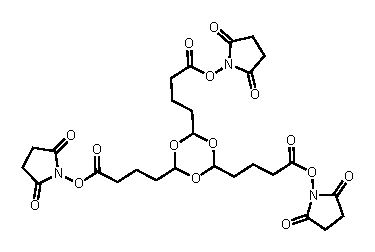
\includegraphics[width=0.4\textwidth]{figures/tri-linker.eps}
    \caption{Structure of TSTO MS cleavable crosslinker with a spacer arm length 
    of 14.0 \AA.}
  \end{figure}
  \begin{block}{}
    For comparison, the commonly used bifunctional crosslinker
  DSSO has a spacer arm length of 10.1 \AA.
    \end{block}
\end{frame}
%----------------------------------------------------------------------------
\begin{frame}
\frametitle{Riccardo's noise model for the crosslinking restraint}
\begin{equation}
p(o_n|X) \propto \frac{\alpha}{\beta}p(XL_n|X) + \frac{1 - \alpha}{1 - \beta}p(\bar{XL_n}|X)
\end{equation}
where 
\begin{equation}
\alpha = \frac{N^{obs, T}_{XL}}{N^{obs}_{XL}} \qquad \beta = \frac{N_{XL}}{N_{LP}}
\end{equation}
For trifunctional crosslinks, the $\beta$ parameter is modified to be 
\begin{equation}
\beta = \frac{N_{XL}^{tri}}{N_{LT}}
\end{equation}
where the number of lysine triplets $N_{LT}$ is 
given by $^{N_{lysines}}C_3 = \frac{N_{lysines}*(N_{lysines}-1)*(N_{lysines}-2)}{3!}$
\end{frame}
%----------------------------------------------------------------------------
\begin{frame}
    \frametitle{Trifunctional XL-MS data processing}
\begin{table}[h]
\centering
\small
\begin{tabular}{llrllr}
\toprule
Protein 1 & Residue 1 & Score 1 & Protein 2 & Residue 2 & Score 2 \\
\midrule
Rpn6  & K141 & 37.7 & Rpn6  & K325 & 22.9 \\
Rpn6  & K288 & 43.3 & Rpn6  & K304 & 51.2 \\
Rpn6  & K288 & 32.8 & Rpn6  & K304 & 45.6 \\
Rpn6  & K288 & 19.4 & Rpn6  & K304 & 48.4 \\
Rpn6  & K288 & 13.9 & Rpn6  & K304 & 43.9 \\
\bottomrule
\end{tabular}
\caption{Example bifunctional crosslinks (N = 3352 total).}
\end{table}
    \begin{table}[h]
\centering
\small
\begin{tabular}{llrllrllr}
\toprule
Protein 1 & Residue 1 & Score 1 & Protein 2 & Residue 2 & Score 2 & Protein 3 & Residue 3 & Score 3 \\
\midrule
Rpn5  & K294 & 12.6 & Rpn5  & K303 & 17.7 & Rpn9  & K132       & 25.6 \\
Rpn5  & K368 & 27.2 & Rpn5  & K376 & 17.4 & Rpn9  & K321;K329  & 31.1 \\
Rpn11 & K152 & 14.9 & Rpn11 & K223 & 19.2 & Rpn8  & K180       & 21.8 \\
Rpn11 & K264 & 40.1 & Rpn7  & K126 & 15.4 & Rpn7  & K163       & 20.6 \\
Rpn11 & K264 & 40.2 & Rpn7  & K126 & 17.4 & Rpn7  & K163       & 16.2 \\
\bottomrule
\end{tabular}
\caption{Example trifunctional crosslinks (N = 216 total).}
\end{table}
\end{frame}
%----------------------------------------------------------------------------
\begin{frame}
\frametitle{Normalizing the ID score}
% side by side figures
\begin{figure}
    \centering
    \begin{subfigure}[b]{0.45\textwidth}
        \centering
        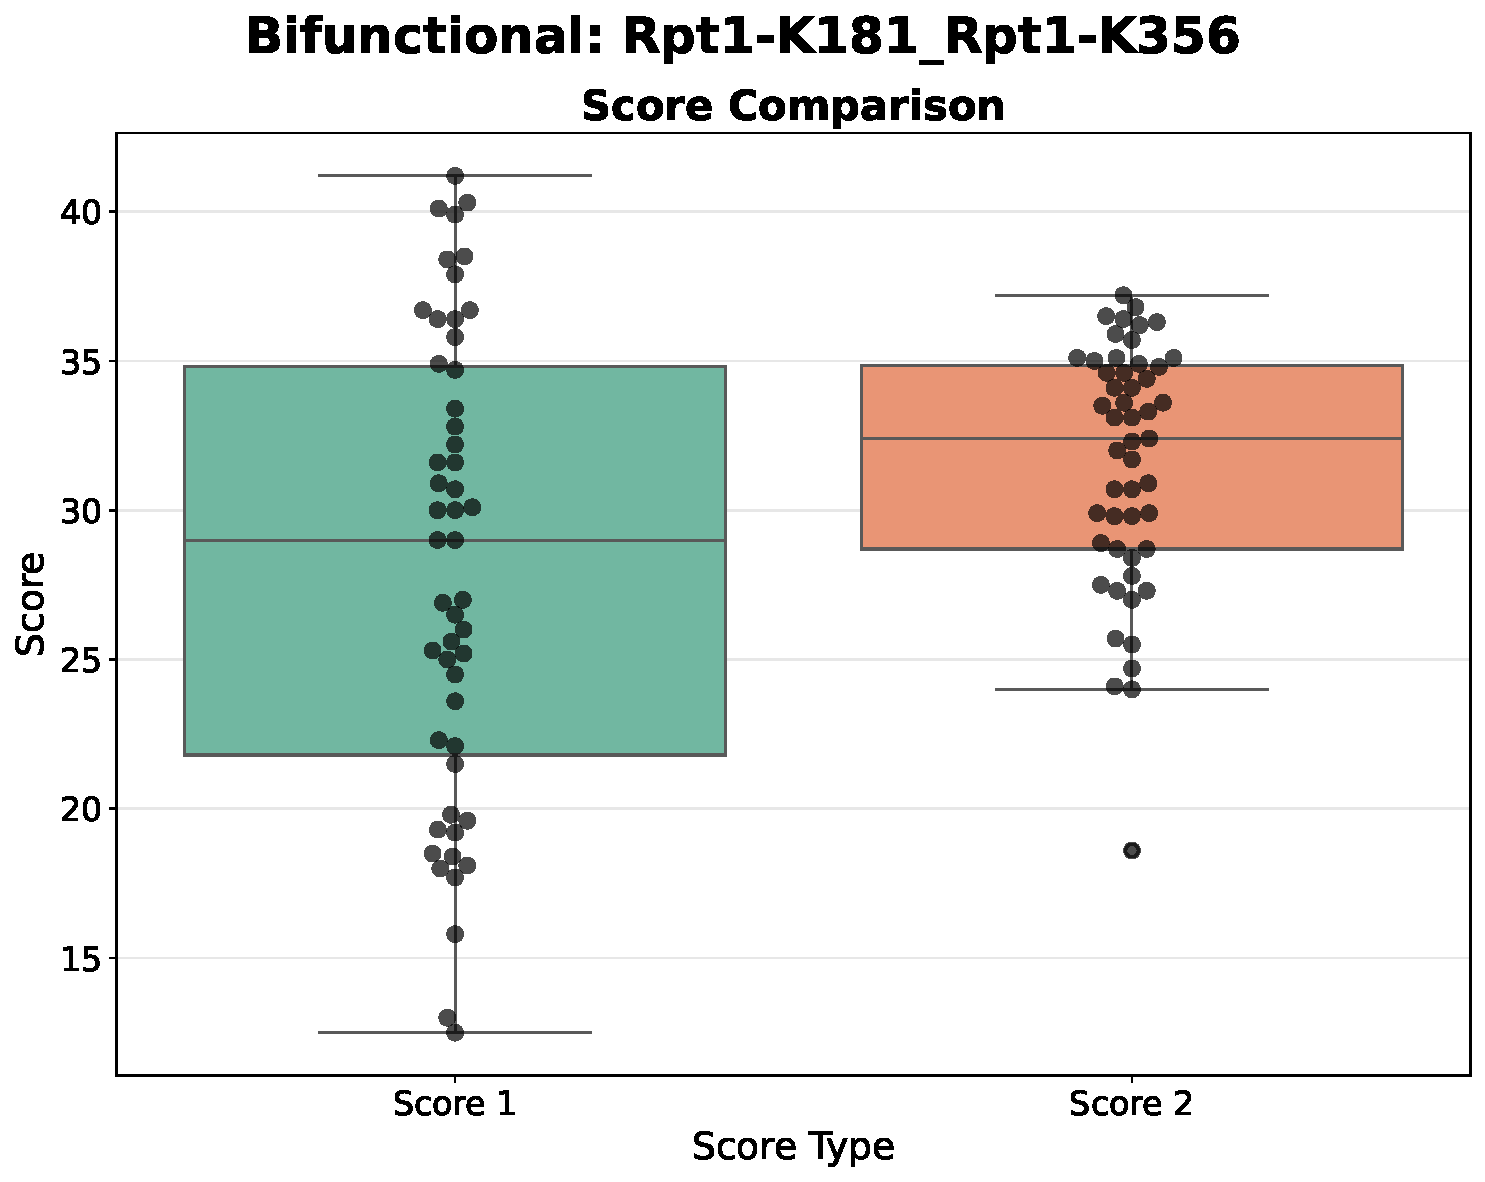
\includegraphics[width=\textwidth]{figures/bifunctional_score_freq.pdf}
        \caption{Raw ID score distribution}
    \end{subfigure}
    \hfill
    \begin{subfigure}[b]{0.45\textwidth}
        \centering
        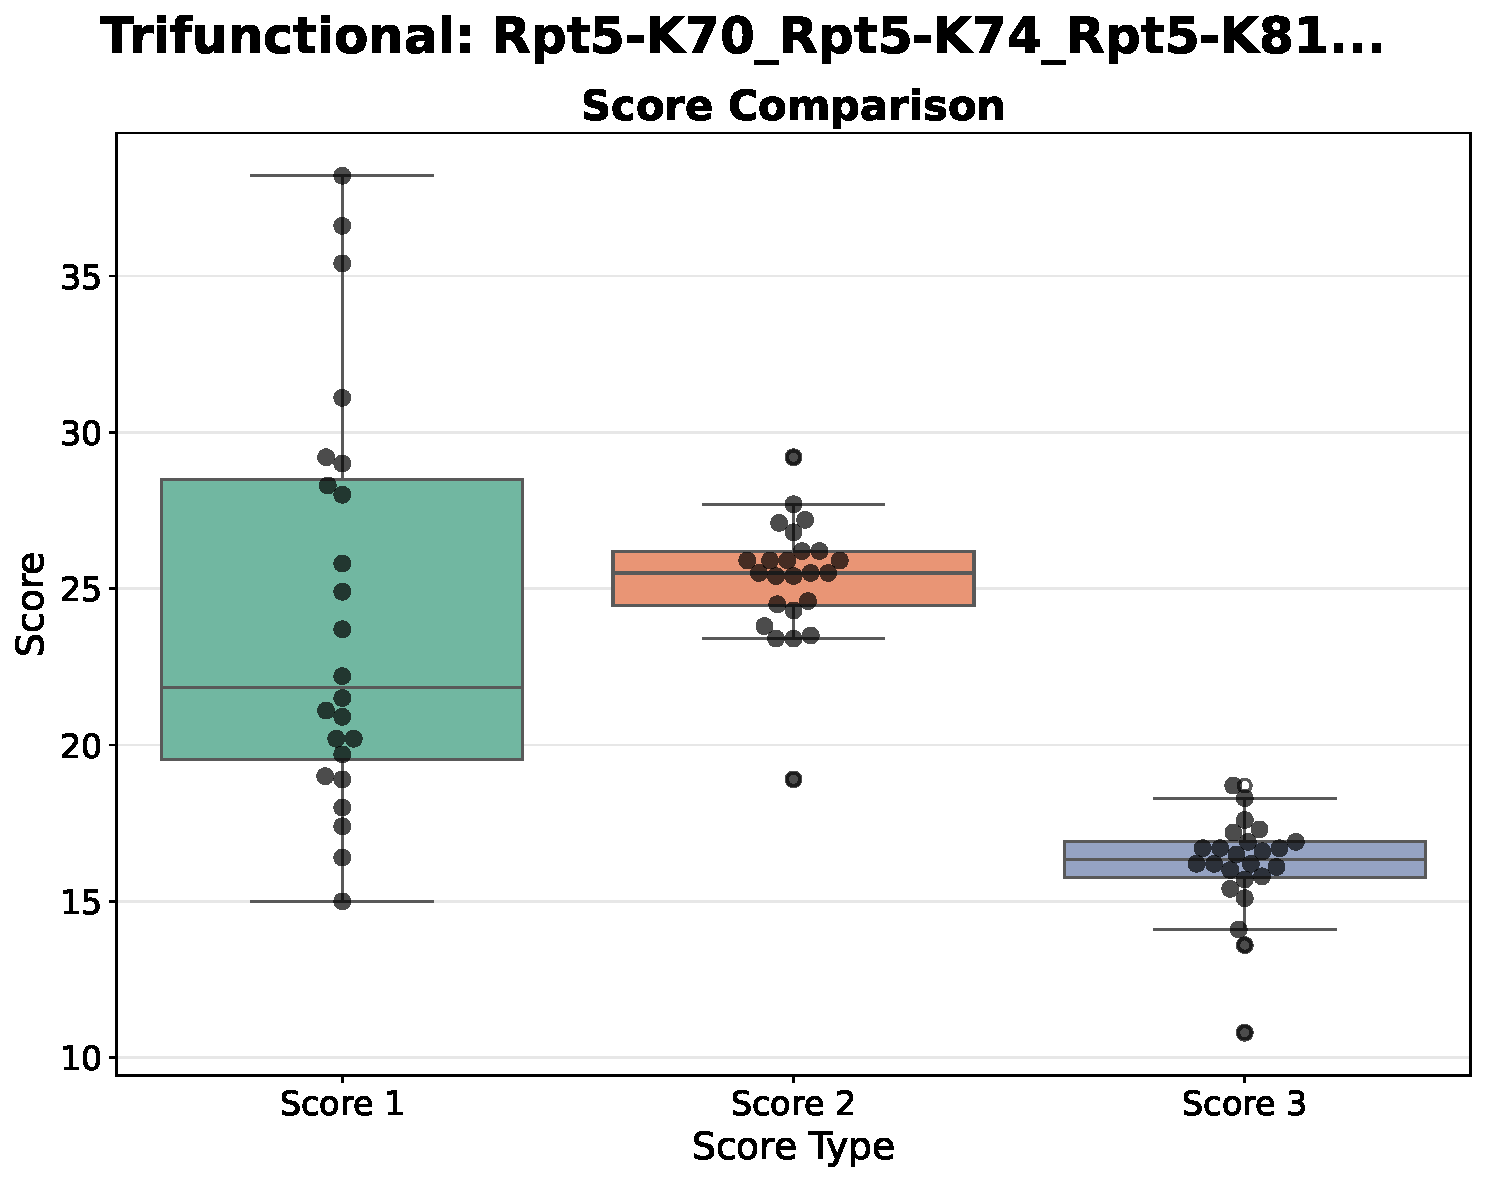
\includegraphics[width=\textwidth]{figures/trifunctional_score_freq.pdf}
        \caption{Normalized ID score distribution}
    \end{subfigure}
    \caption{Distributions of raw and normalized ID scores for trifunctional crosslinks.}
\end{figure}
\end{frame}

\begin{frame}{Noise model: extending Riccardo's bifunctional model to trifunctional crosslinks}
    
    \begin{columns}
    
        \begin{column}{0.45\textwidth}
            \begin{block}{1. Create "Ground Truth"}
                \begin{itemize}
                    \item Create 10,000 particles in a 3D box.
                    \item Define "True" geometry: A triplet (A,B,C) is satisfied if all distances ($d_{ab}, d_{ac}, d_{bc}$) are $< 25$ \AA.
                \end{itemize}
            \end{block}
            
            \begin{block}{2. Generate "Perfect" Data}
                \begin{itemize}
                    \item Find 140 triplets that satisfy the true geometry. These are our True Positives (TPs).
                \end{itemize}
            \end{block}
        \end{column}
    
        \begin{column}{0.45\textwidth}
            \begin{block}{3. Corrupt the Data (Add Noise)}
                \begin{itemize}
                    \item \textbf{Over-length TPs (28):} Take 20% of TPs and add noise to one distance, making it "too long" (e.g., $d_{bc}' = d_{bc} + \mathcal{N}(0, 10\AA)$).
                    \item \textbf{False Positives (60):} Add 60 completely random triplets.
                \end{itemize}
            \end{block}
            
            \begin{block}{4. Simulate ID Scores}
                \begin{itemize}
                    \item Assign \textbf{high scores} (e.g., 0.7-1.0) to all TPs (both good and over-length).
                    \item Assign \textbf{low scores} (e.g., 0.0-0.4) to all FPs.
                \end{itemize}
            \end{block}
        \end{column}
        
    \end{columns}

\end{frame}

\begin{frame}
    \frametitle{Forward model: Extension to trifunctional crosslinks}
    \begin{block}{}
        Forward model for bifunctional crosslinks 
        \begin{itemize}
            \item Consider the coordinates of coarse grained beads (residues) $\vec{r1}$ and $\vec{r2}$ connected by a bifunctional crosslinker.
            \item The uncertainty in the C$-\alpha$ atom position can be modeled using a sphere around the bead defined by $\sigma1$ and
            $\sigma2$ respectively.
            \item The distance between the centers of the spheres is $d = ||\vec{r1} - \vec{r2}||$.
            \item The probability that the crosslink is satisfied (i.e., the two residues are within the crosslinker length 
            $l_{xl}$) is to be computed, geometrically the problem is simplified as finding the volume of intersection of two spheres,
            the spheres representing the uncertainty in the position of the two residues        
        \end{itemize}

        \end{block}
\end{frame}
%----------------------------------------------------------------------------
\begin{frame}
\frametitle{Model problem}
\begin{figure}
    \centering
    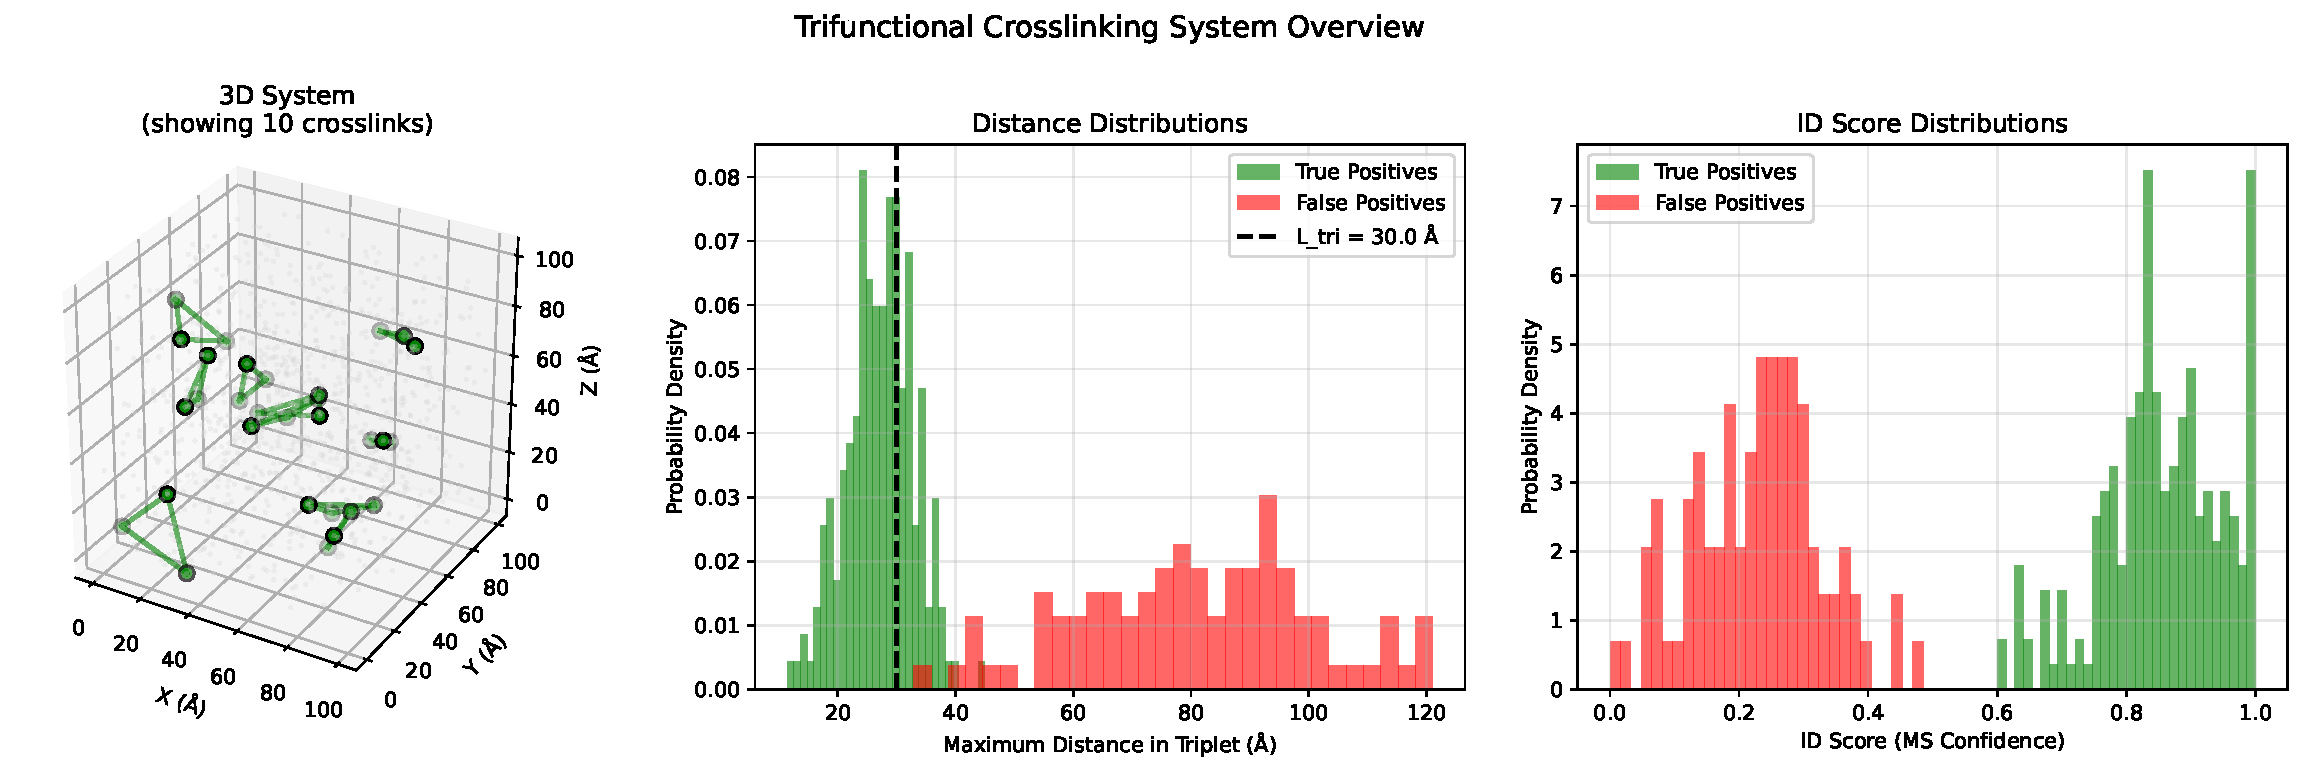
\includegraphics[width=0.6\textwidth]{figures/crosslinking_system.pdf}
    \caption{Schematic of the model problem setup}
\end{figure}
\end{frame}
%----------------------------------------------------------------------------
%----------------------------------------------------------------------------
\begin{frame}
\frametitle{Slide 1: Model Problem Setup}
\begin{block}{Physical System}
    \begin{itemize}
        \item \textbf{N = 1000 particles} randomly distributed in a 100×100×100 ų box
        \item \textbf{Trifunctional crosslinker}: connects 3 particles (A, B, C)
        \item \textbf{Geometric constraint}: All three pairwise distances must satisfy:
        \begin{equation*}
            d_{AB} < L_{tri}, \quad d_{AC} < L_{tri}, \quad d_{BC} < L_{tri}
        \end{equation*}
        where $L_{tri} = 30$ Å (maximum arm length)
    \end{itemize}
\end{block}

\begin{block}{Key Parameters (Ground Truth)}
    \begin{itemize}
        \item $\sigma = 5.0$ Å: Distance measurement uncertainty
        \item FP rate = 30\%: Fraction of false positive crosslinks
        \item Total crosslinks: 300 (210 TPs, 90 FPs)
    \end{itemize}
\end{block}
\end{frame}

%----------------------------------------------------------------------------
\begin{frame}
\frametitle{Slide 2: Synthetic Data Generation}
\begin{columns}
\begin{column}{0.5\textwidth}
    \begin{block}{True Positives (70\%)}
        \begin{enumerate}
            \item Sample random particle triplets
            \item Check geometric constraint:
            \begin{equation*}
                d_{AB}, d_{AC}, d_{BC} < 30\text{ Å}
            \end{equation*}
            \item Add Gaussian noise: $d_{obs} = d_{true} + \mathcal{N}(0, \sigma)$
            \item Assign high ID scores: $\mathcal{N}(0.85, 0.1)$
        \end{enumerate}
    \end{block}
\end{column}

\begin{column}{0.5\textwidth}
    \begin{block}{False Positives (30\%)}
        \begin{enumerate}
            \item Sample completely random triplets (no geometric check)
            \item Use observed distances directly
            \item Assign low ID scores: $\mathcal{N}(0.25, 0.1)$
        \end{enumerate}
    \end{block}
    
    \vspace{0.5cm}
    
    \begin{highlightbox}
        \textbf{Result}: 300 crosslinks with known ground truth labels for validation
    \end{highlightbox}
\end{column}
\end{columns}
\end{frame}

%----------------------------------------------------------------------------
\begin{frame}
\frametitle{Slide 3: Beta Parameter - Random Match Probability}
\begin{block}{Definition}
    $\beta$ = Probability that a randomly selected triplet satisfies all geometric constraints
\end{block}

\begin{block}{Empirical Calculation}
    \begin{enumerate}
        \item Sample 100,000 random particle triplets
        \item Count how many satisfy: $d_{AB}, d_{AC}, d_{BC} < L_{tri}$
        \item Calculate: $\beta_{empirical} = \frac{\text{satisfied triplets}}{100,000}$
    \end{enumerate}
    
    \vspace{0.3cm}
    For our system: \textbf{$\beta \approx 0.027$} (2.7\% of random triplets satisfy constraints)
\end{block}

\begin{block}{Theoretical Estimate}
    Assuming uniform distribution:
    \begin{equation*}
        \beta_{theoretical} \approx \left(\frac{L_{tri}}{BOX\_SIZE}\right)^3 = \left(\frac{30}{100}\right)^3 = 0.027
    \end{equation*}
    Good agreement with empirical calculation!
\end{block}
\end{frame}

%----------------------------------------------------------------------------
\begin{frame}
\frametitle{Slide 4: Alpha Calibration via Isotonic-like Regression}
\begin{columns}
\begin{column}{0.55\textwidth}
    \begin{block}{Motivation}
        \begin{itemize}
            \item ID scores are not calibrated probabilities
            \item Need mapping: ID score $\rightarrow$ precision ($\alpha$)
            \item Constraint: higher ID score $\Rightarrow$ higher precision
        \end{itemize}
    \end{block}
    
    \begin{block}{Smooth Logistic Model}
        \begin{equation*}
            \alpha(s) = \text{sigmoid}(\beta_0 + \beta_1 \cdot s)
        \end{equation*}
        where:
        \begin{itemize}
            \item $s$ = ID score (0 to 1)
            \item $\beta_0$ = intercept (prior: $\mathcal{N}(-2, 1)$)
            \item $\beta_1$ = slope (prior: Half-Normal(5))
        \end{itemize}
    \end{block}
\end{column}

\begin{column}{0.45\textwidth}
    \begin{figure}
        \centering
        \includegraphics[width=\textwidth]{figures/calibration_curve_example.pdf}
        \caption{Calibration curve mapping ID scores to precision}
    \end{figure}
\end{column}
\end{columns}
\end{frame}

%----------------------------------------------------------------------------
\begin{frame}
\frametitle{Slide 5: Bayesian Inference via HMC/NUTS}
\begin{block}{Model Structure}
    \textbf{Priors:}
    \begin{align*}
        \sigma &\sim \text{Half-Normal}(10) \\
        \beta_0 &\sim \mathcal{N}(-2, 1) \\
        \beta_1 &\sim \text{Half-Normal}(5)
    \end{align*}
    
    \textbf{Likelihood:}
    \begin{equation*}
        p(obs|params) = \alpha(s) \cdot p_{TP} + (1-\alpha(s)) \cdot \beta
    \end{equation*}
    where $p_{TP} = \text{sigmoid}\left(\frac{L_{tri} - d_{AB}}{\sigma}\right) \cdot \text{sigmoid}\left(\frac{L_{tri} - d_{AC}}{\sigma}\right) \cdot \text{sigmoid}\left(\frac{L_{tri} - d_{BC}}{\sigma}\right)$
\end{block}

\begin{block}{MCMC Sampling}
    \begin{itemize}
        \item Sampler: NUTS (No-U-Turn Sampler) - adaptive HMC
        \item 3000 draws $\times$ 4 chains, 2000 tuning steps
        \item Target acceptance rate: 0.95 (high to avoid divergences)
    \end{itemize}
\end{block}
\end{frame}

%----------------------------------------------------------------------------
\begin{frame}
\frametitle{Slide 6: Results and Validation}
\begin{columns}
\begin{column}{0.5\textwidth}
    \begin{block}{Parameter Recovery}
        \begin{table}
        \small
        \begin{tabular}{lcc}
        \toprule
        Parameter & True & Inferred \\
        \midrule
        $\sigma$ (Å) & 5.0 & 5.2 ± 0.3 \\
        \bottomrule
        \end{tabular}
        \end{table}
        
        \textbf{Convergence:}
        \begin{itemize}
            \item $\hat{R} < 1.01$ for all parameters
            \item ESS $>$ 400 (effective sample size)
        \end{itemize}
    \end{block}
\end{column}

\begin{column}{0.5\textwidth}
    \begin{block}{Classification Performance}
        Using $\alpha > 0.5$ as TP cutoff:
        \begin{table}
        \small
        \begin{tabular}{lc}
        \toprule
        Metric & Value \\
        \midrule
        Accuracy & 0.89 \\
        Precision & 0.92 \\
        Recall & 0.91 \\
        F1 Score & 0.91 \\
        \bottomrule
        \end{tabular}
        \end{table}
    \end{block}
\end{column}
\end{columns}

\vspace{0.3cm}

\begin{highlightbox}
    \textbf{Key Result}: The model successfully recovers $\sigma$ and correctly classifies 89\% of crosslinks using only ID scores and geometric constraints!
\end{highlightbox}
\end{frame}
\end{document}
%**********************************************************************
